\chapter{Exploratory Data Analysis}

\section{Overview}
Before building models, it is essential to understand the underlying distributions and spectral characteristics of the dataset. EDA provides the intuition required for intelligent feature engineering.

\section{Class Distribution Analysis}
As highlighted in the preprocessing section, the dataset is heavily skewed toward "Normal" operation. This reflects real-world industrial conditions where machines spend the majority of their time in a healthy state. The overall ratio observed is approximately 5:1 (Normal to Abnormal), which necessitates the use of class weighting in the final classification models.

\begin{figure}[H]
    \centering
    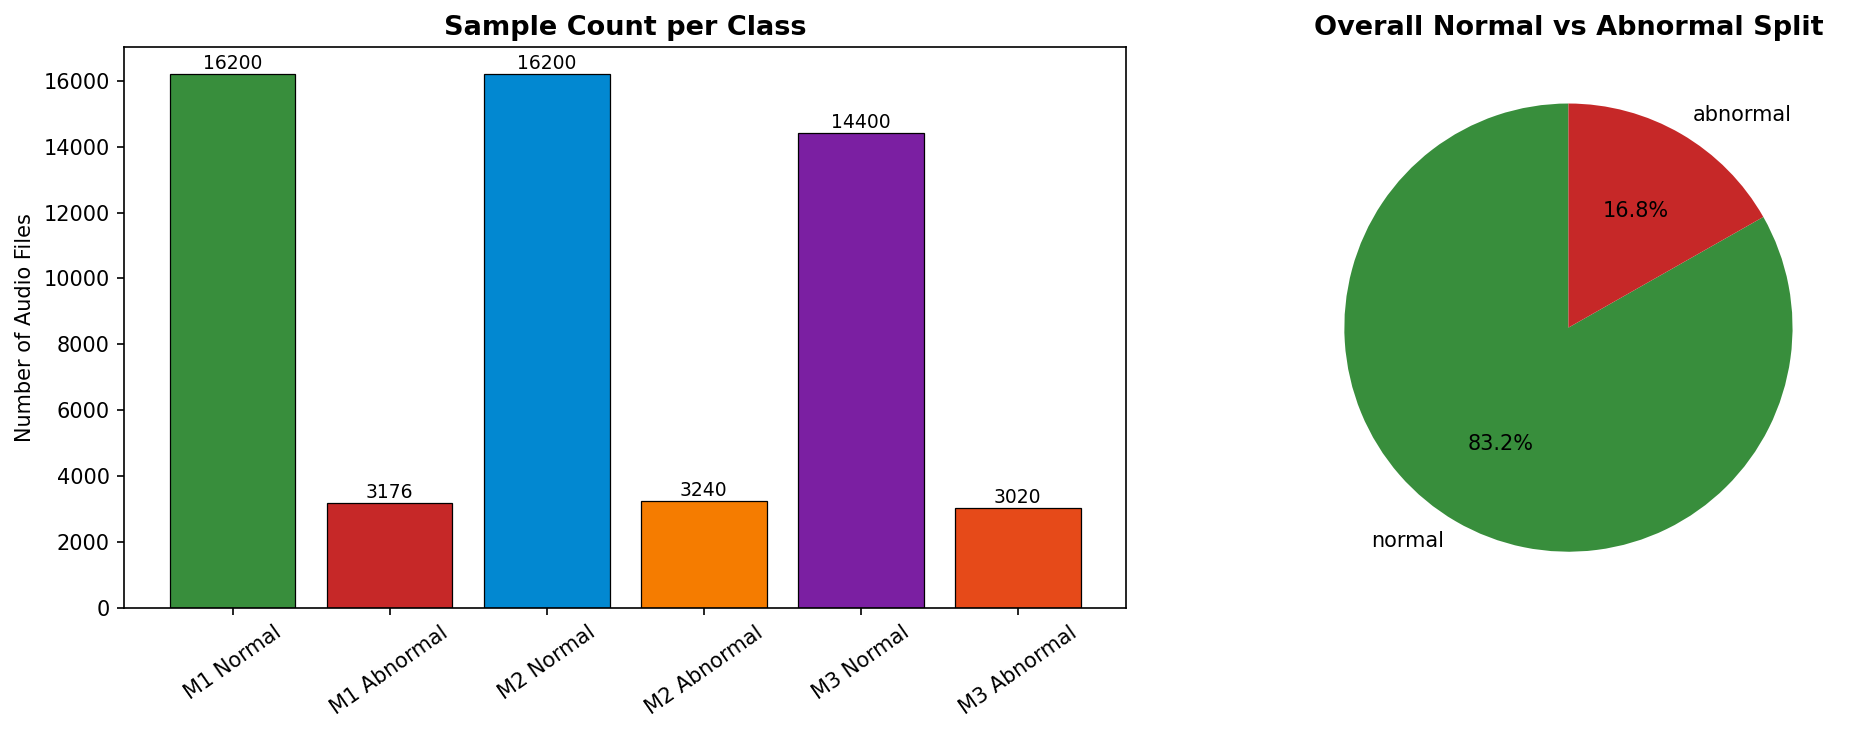
\includegraphics[width=0.7\textwidth]{figures/eda_class_balance.png}
    \caption{Class Balance across Machines 1, 2, and 3 (Normal vs. Abnormal)}
    \label{fig:class_dist}
\end{figure}

The dataset exhibits a consistent 5:1 ratio of Normal to Abnormal recordings across all three machines. This inherent class imbalance across the entire dataset is the primary factor that influenced our decision to prioritize the Macro F1-score as our evaluation metric.

\section{Temporal and Spectral Distributions}
Detailed metadata analysis confirms that 100\% of the dataset is recorded at a uniform sample rate of 48 kHz. However, audio durations are discrete and machine-dependent: Machine 1 and 2 are exactly 11.0 seconds, while Machine 3 is exactly 10.0 seconds. 

\begin{figure}[H]
    \centering
    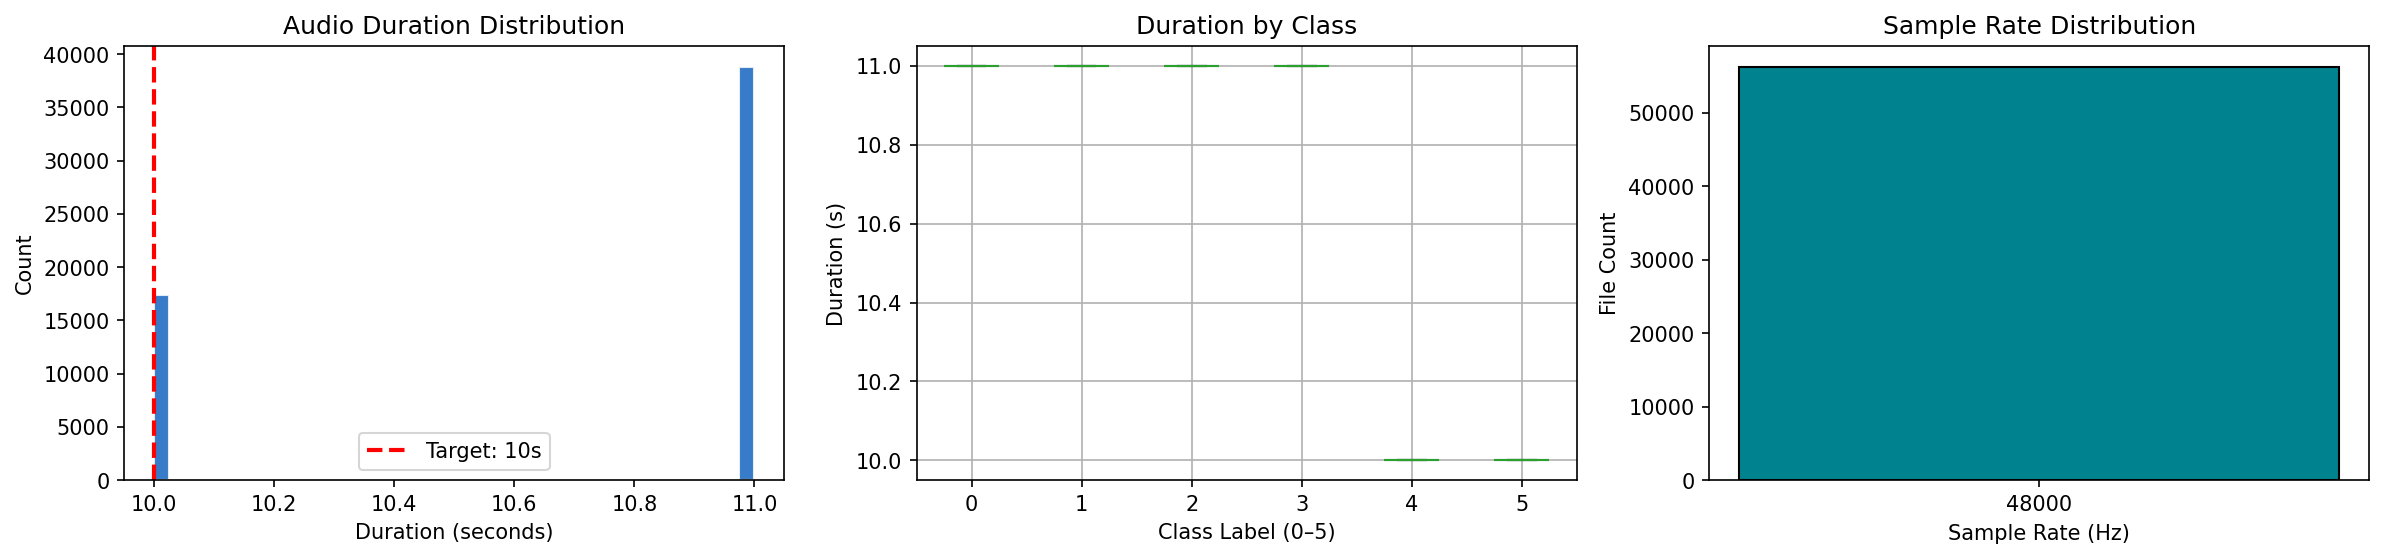
\includegraphics[width=0.7\textwidth]{figures/eda_duration_sr.png}
    \caption{Distribution of Recording Durations and Sample Rates}
    \label{fig:duration_sr}
\end{figure}

To handle this variability, our pipeline pads all recordings to a fixed 11-second window, ensuring that the critical "end-of-cycle" anomalies in Machines 1 and 2 are never truncated.

\section{Spectral and Waveform Comparison}
By comparing the raw waveforms and Mel-spectrograms of normal and abnormal recordings, we can identify visual patterns in the acoustic frequency domain. 

\begin{figure}[H]
    \centering
    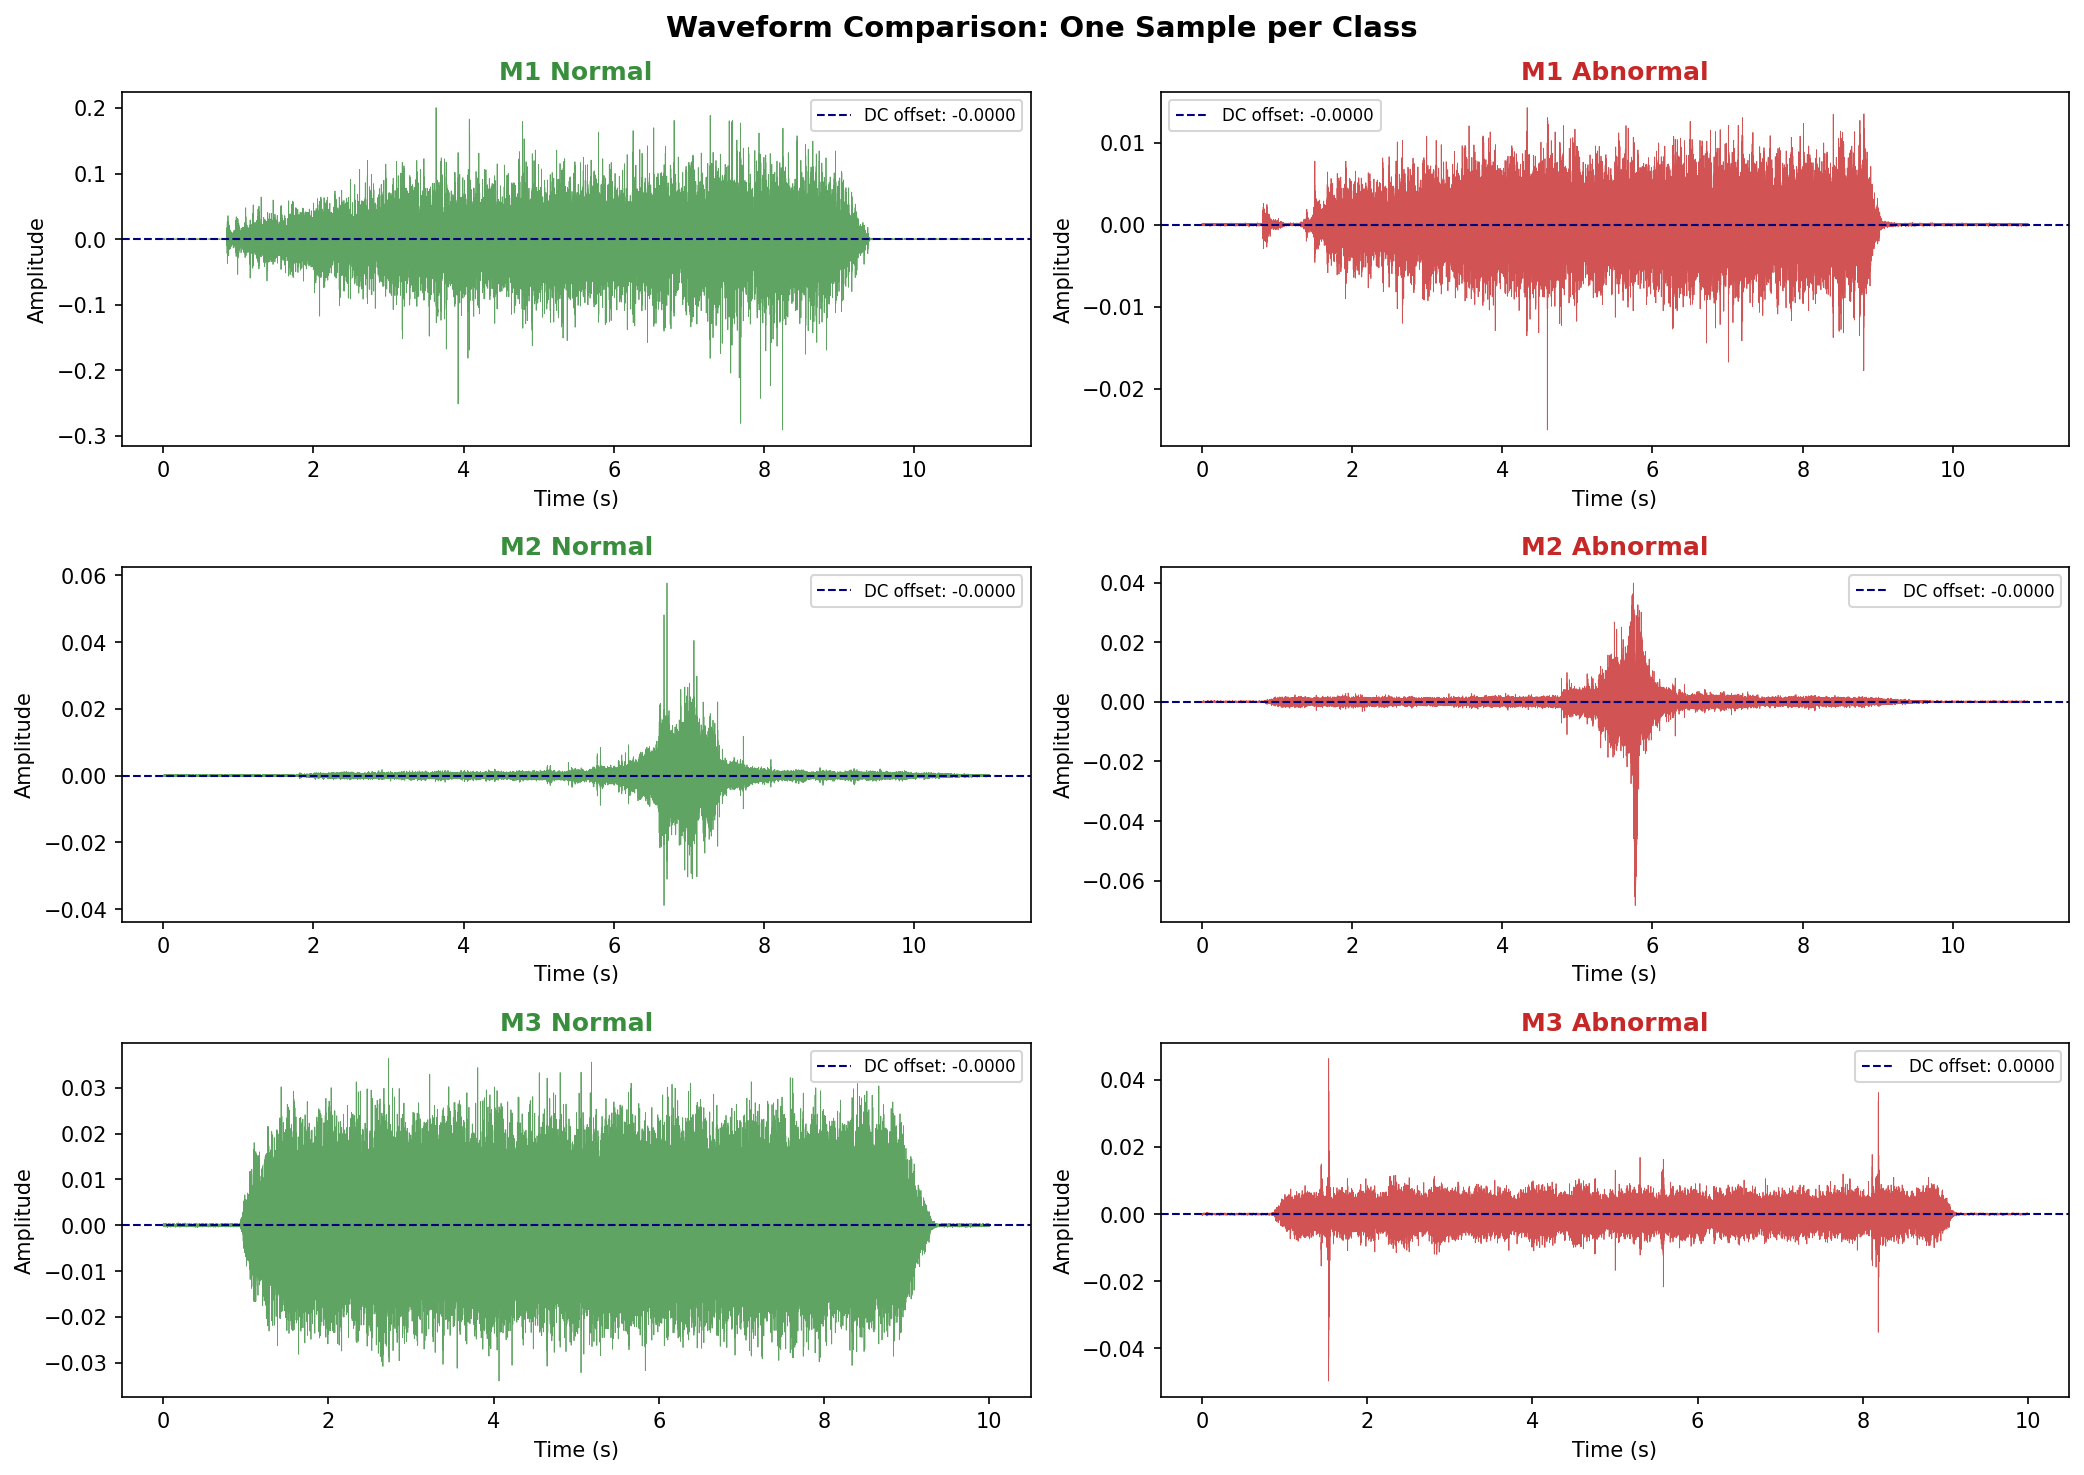
\includegraphics[width=0.75\textwidth]{figures/eda_waveforms.png}
    \caption{Time-Domain Waveform Comparison (Normal vs. Abnormal)}
    \label{fig:waveforms}
\end{figure}

\begin{figure}[H]
    \centering
    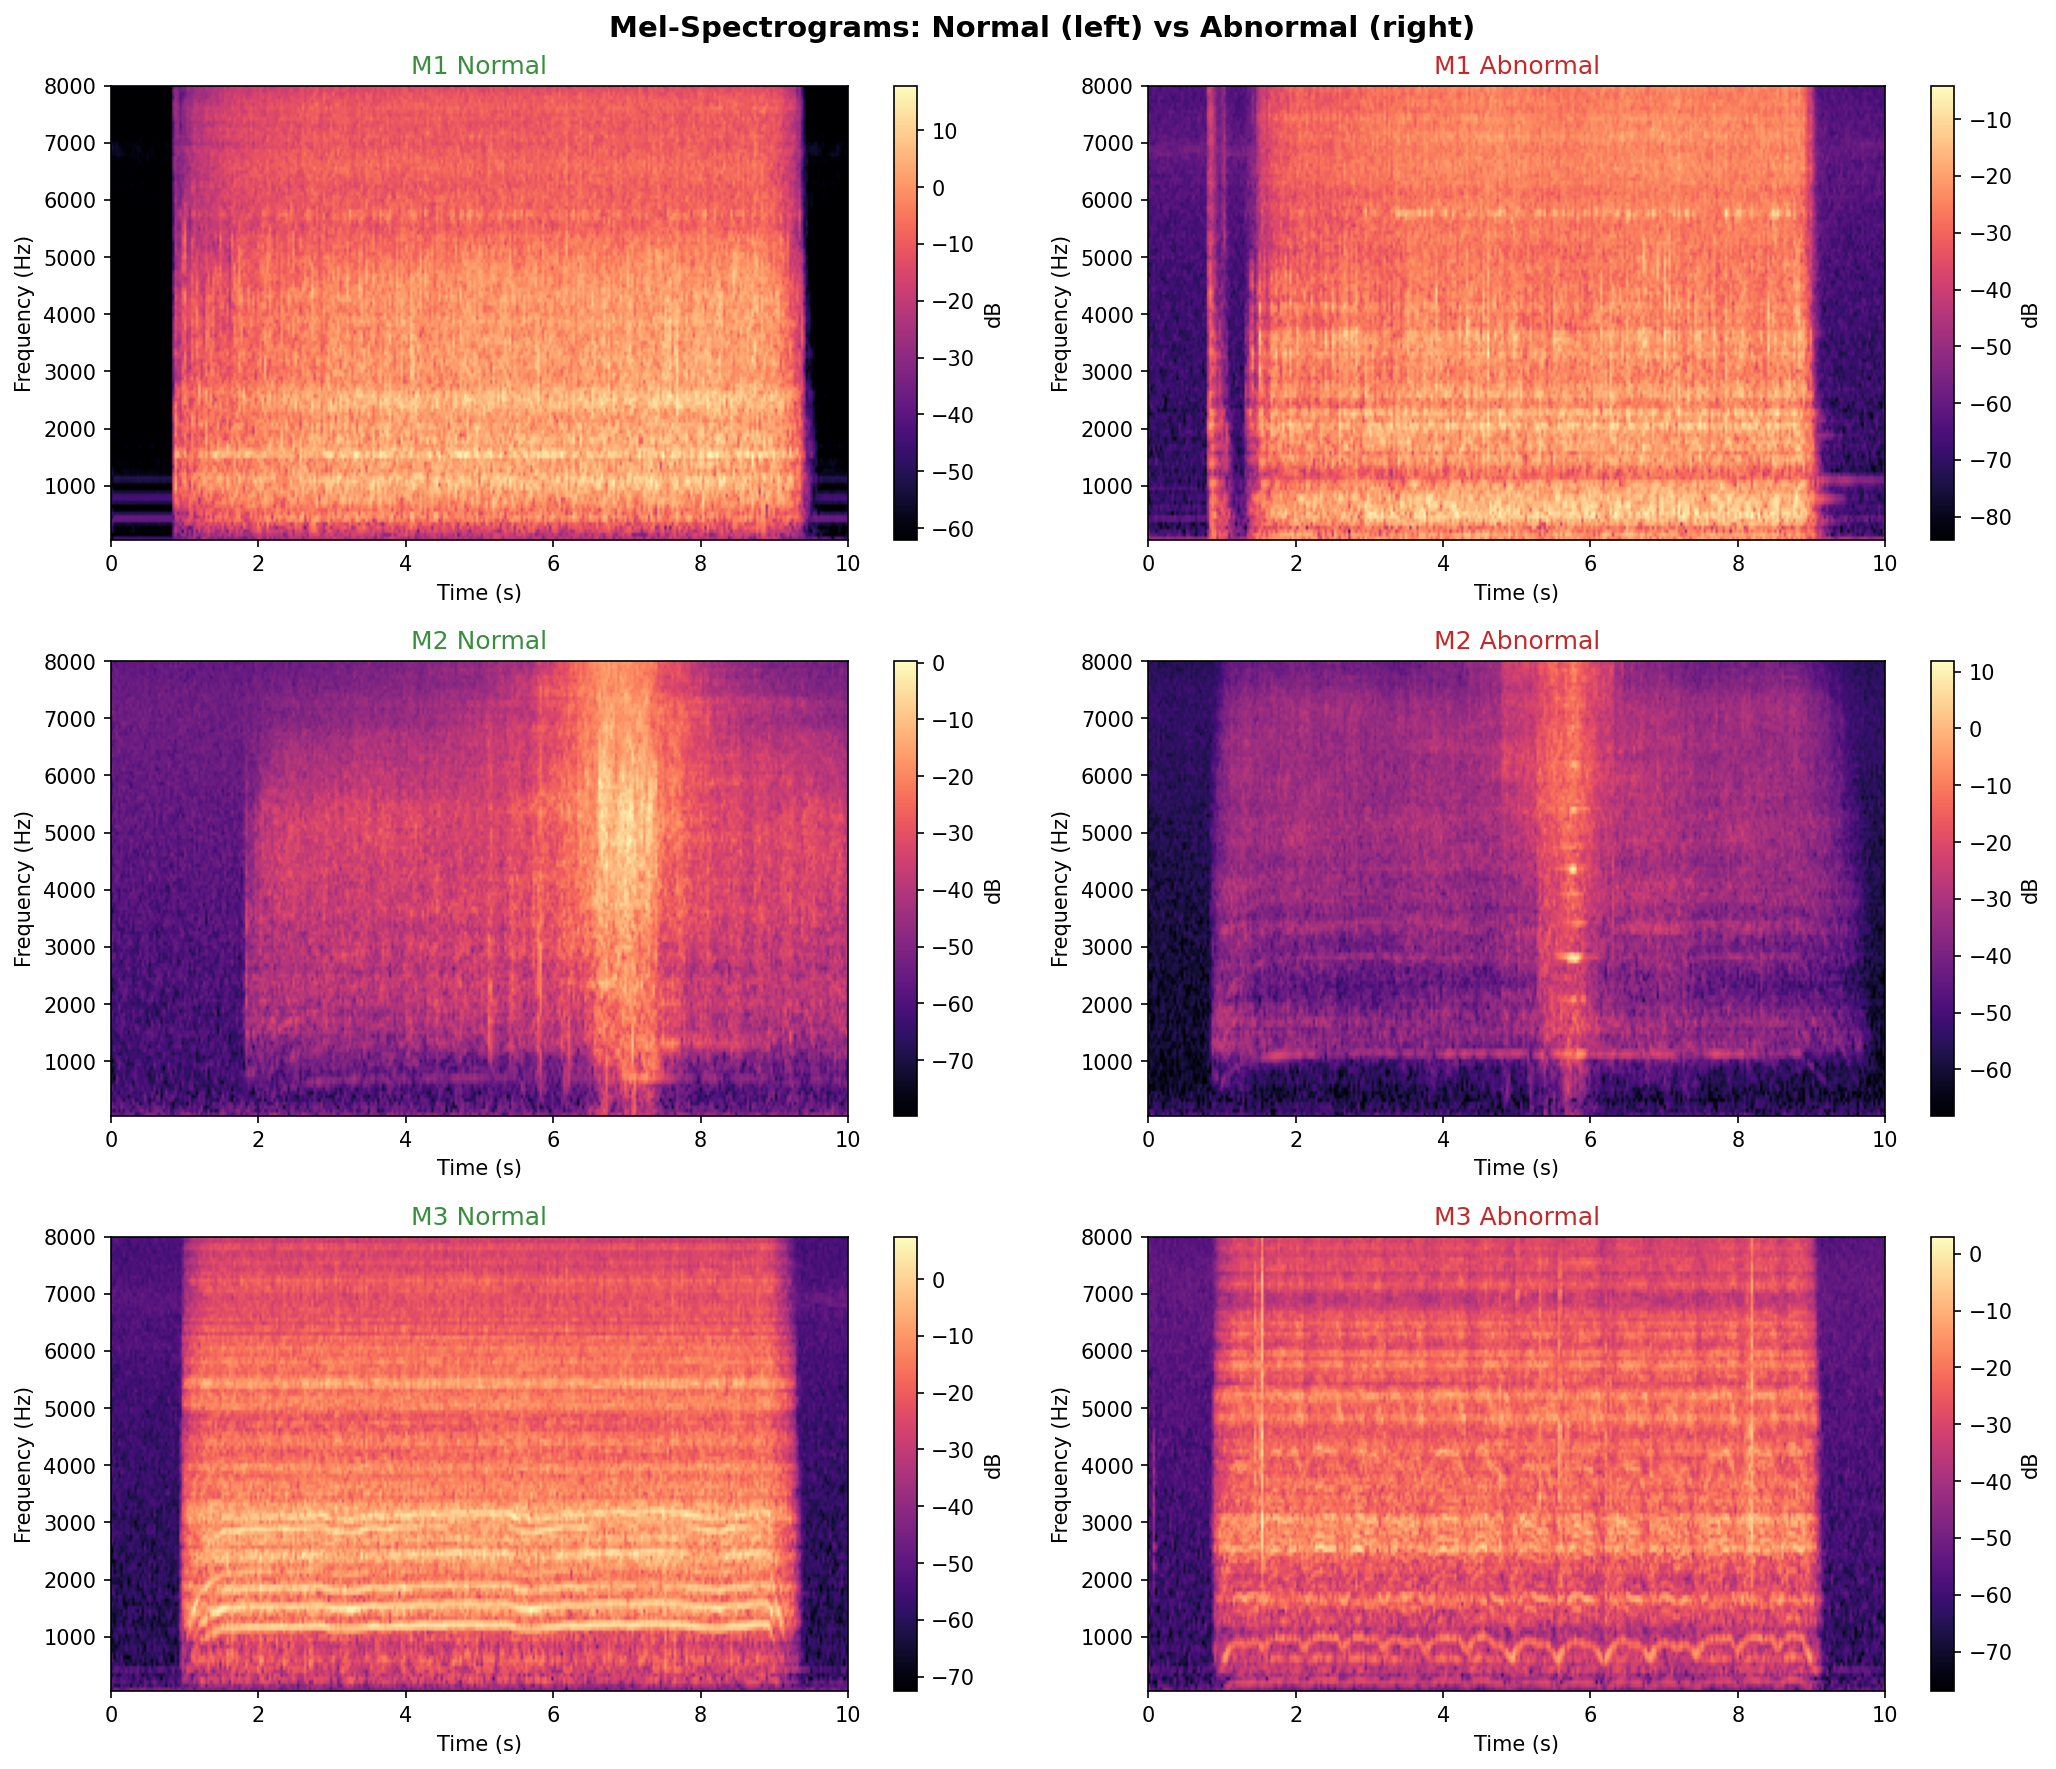
\includegraphics[width=0.75\textwidth]{figures/eda_spectrograms.png}
    \caption{Mel-Spectrogram Visual Signatures}
    \label{fig:spectrograms}
\end{figure}

\subsection{Normal Acoustic Signatures}
Normal recordings are characterized by stable, periodic harmonic structures. In Machines 1 and 2, the spectrogram shows consistent horizontal bands representing the fundamental frequency and its overtones, corresponding to constant rotation speeds.

\subsection{Abnormal Acoustic Signatures}
Anomalies often manifest as transient energy bursts or broadband noise. General patterns observed across the dataset include:
\begin{itemize}
    \item \textbf{Impulse Noise:} High-intensity vertical streaks indicating clashing components or gear teeth chipping.
    \item \textbf{Harmonic Shift:} Changes in the overtone structure, often indicating mechanical loose-fit or bearing degradation.
    \item \textbf{Signal-to-Noise Ratio (SNR) Drops:} Abnormal states frequently show a higher noise floor across all frequencies compared to normal states.
\end{itemize}

\begin{figure}[H]
    \centering
    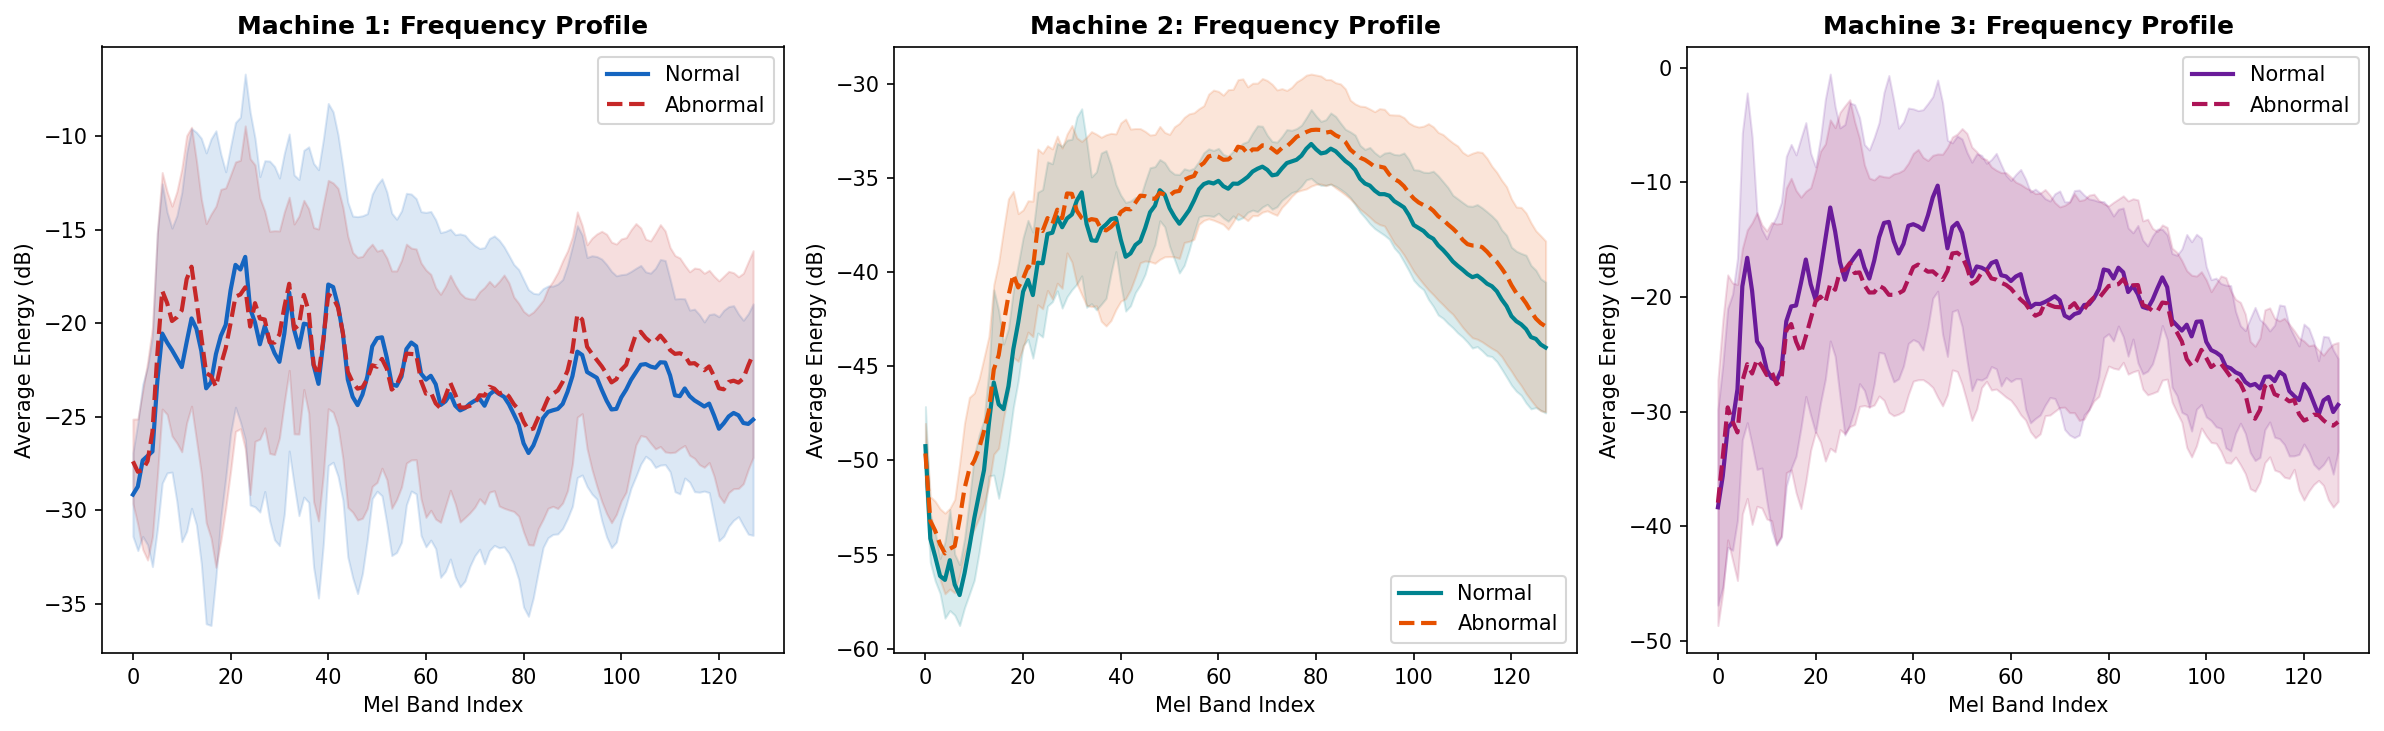
\includegraphics[width=0.8\textwidth]{figures/eda_freq_profiles.png}
    \caption{Frequency Band Profiles across Machines}
    \label{fig:freq_profiles}
\end{figure}

\begin{figure}[H]
    \centering
    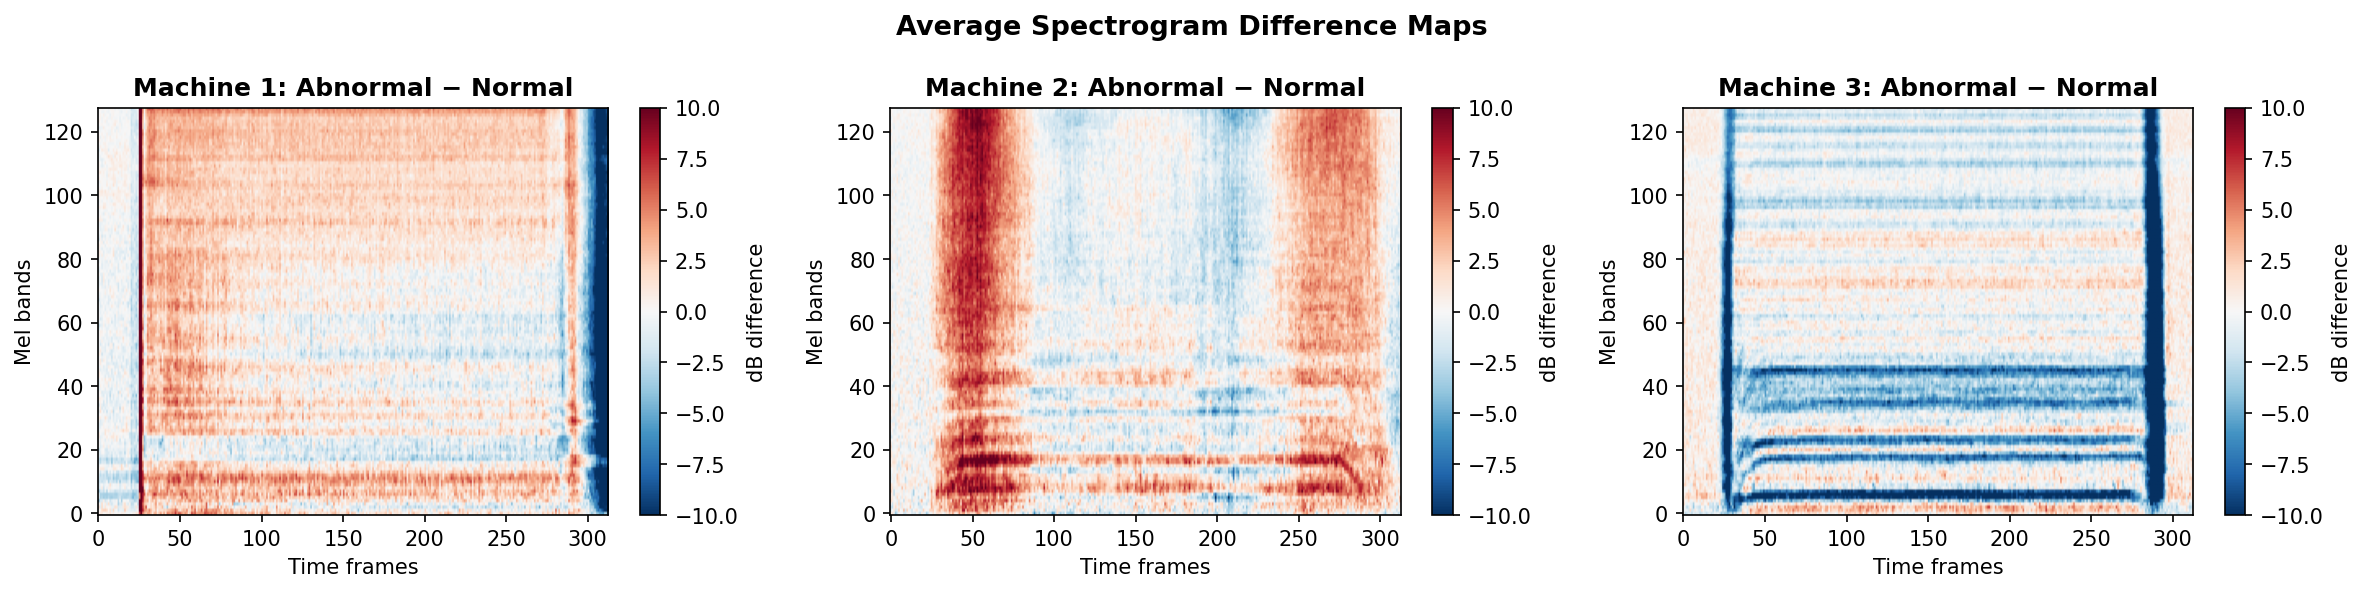
\includegraphics[width=0.8\textwidth]{figures/eda_diff_maps.png}
    \caption{Spectral Difference Maps (Abnormal - Normal)}
    \label{fig:diff_maps}
\end{figure}

\section{RMS Energy and Statistical Significance}
Mann-Whitney U Tests confirm that the difference in RMS Energy between Normal and Abnormal states is highly statistically significant ($p < 0.001$) across all machines. This justifies our decision to prohibit per-file normalization, as absolute volume is a critical feature.

\begin{figure}[H]
    \centering
    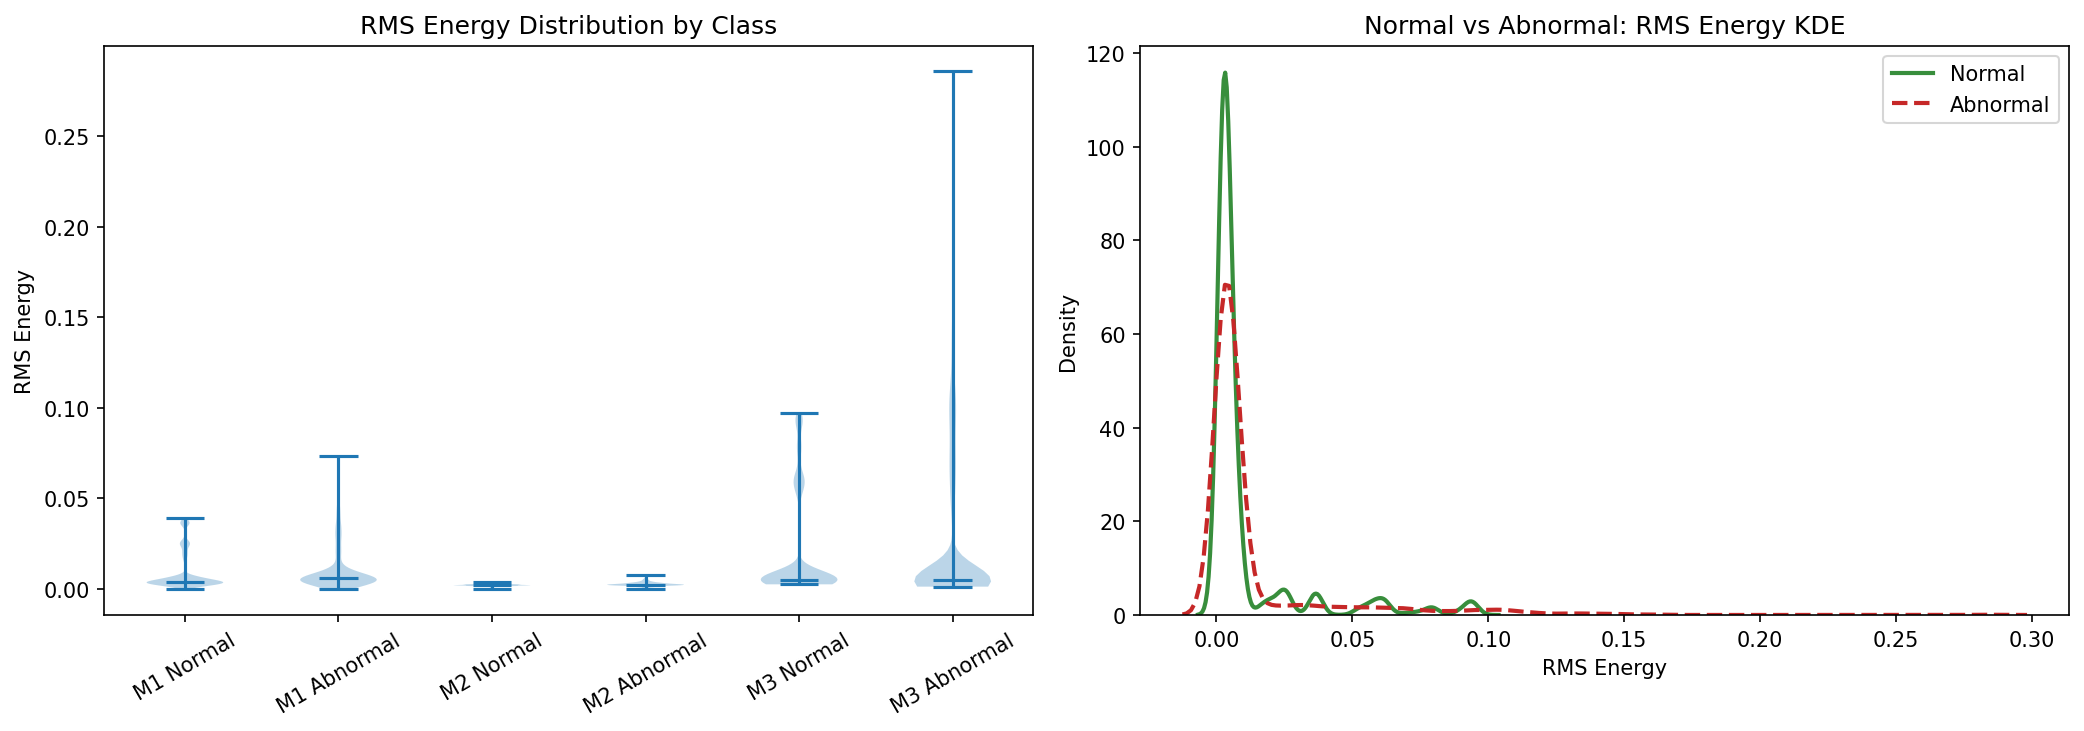
\includegraphics[width=0.7\textwidth]{figures/eda_energy.png}
    \caption{RMS Energy Distribution (Statistically Significant Separation)}
    \label{fig:energy_dist}
\end{figure}

\section{Outliers and Data Quality}
Exactly 142 files (0.3\% of the dataset) exhibited extreme energy z-scores > 3. These represent catastrophic mechanical faults that must be preserved for training rather than clipped as noise.

\begin{figure}[H]
    \centering
    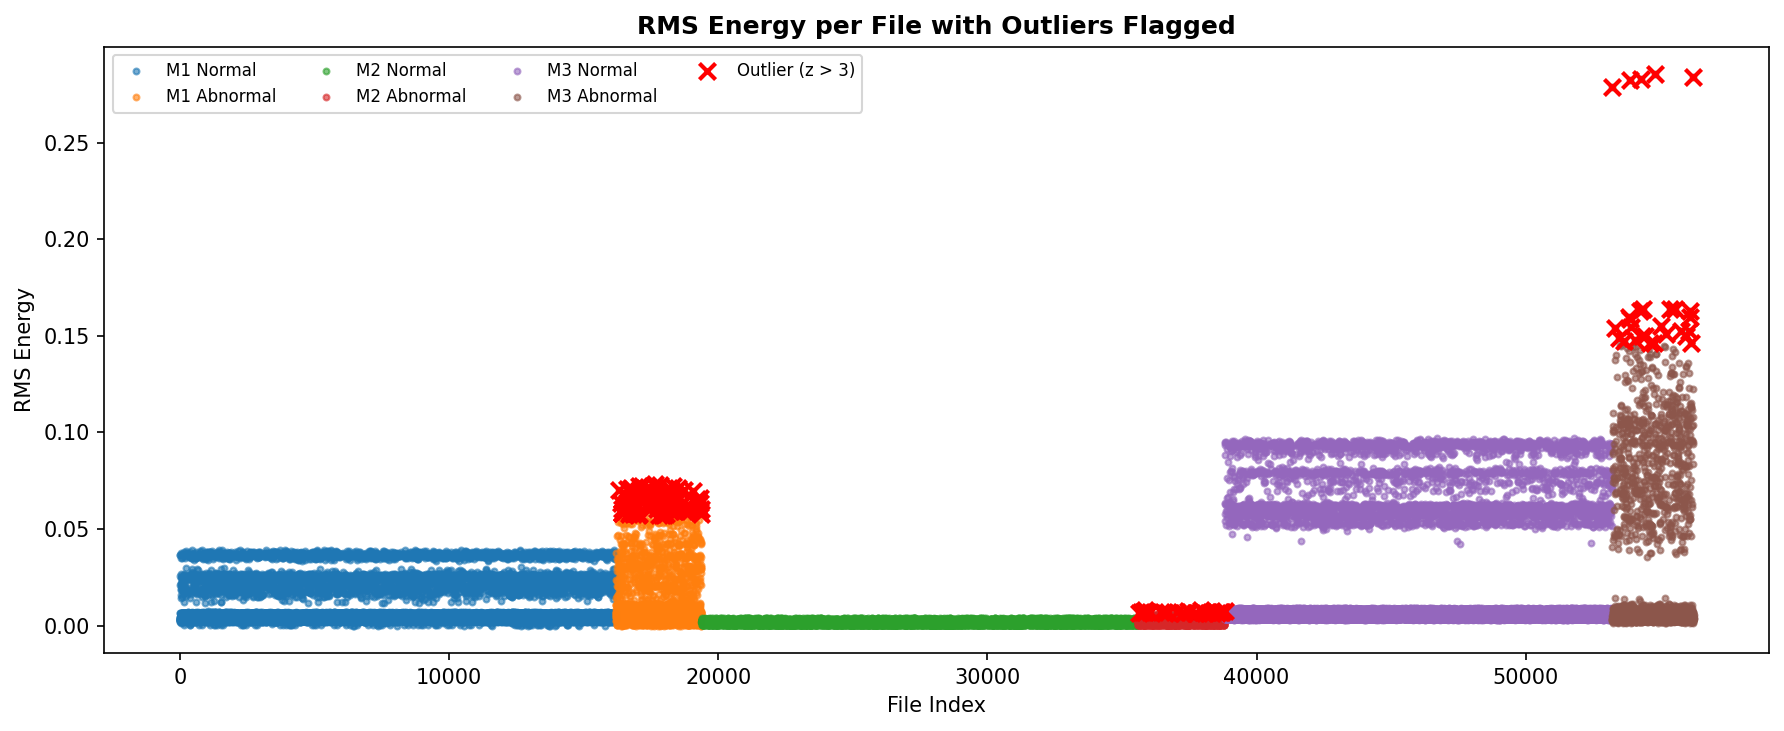
\includegraphics[width=0.7\textwidth]{figures/eda_outliers.png}
    \caption{Identification of High-Energy Acoustic Outliers}
    \label{fig:outliers}
\end{figure}

\section{Silence Ratio and Background Noise}
The dataset exhibits a high overall silence ratio (mean = 0.86), particularly in Machine 2. This confirms that anomalies are highly localized in time, necessitating the use of temporal attention in our Deep Learning architecture.

\begin{figure}[H]
    \centering
    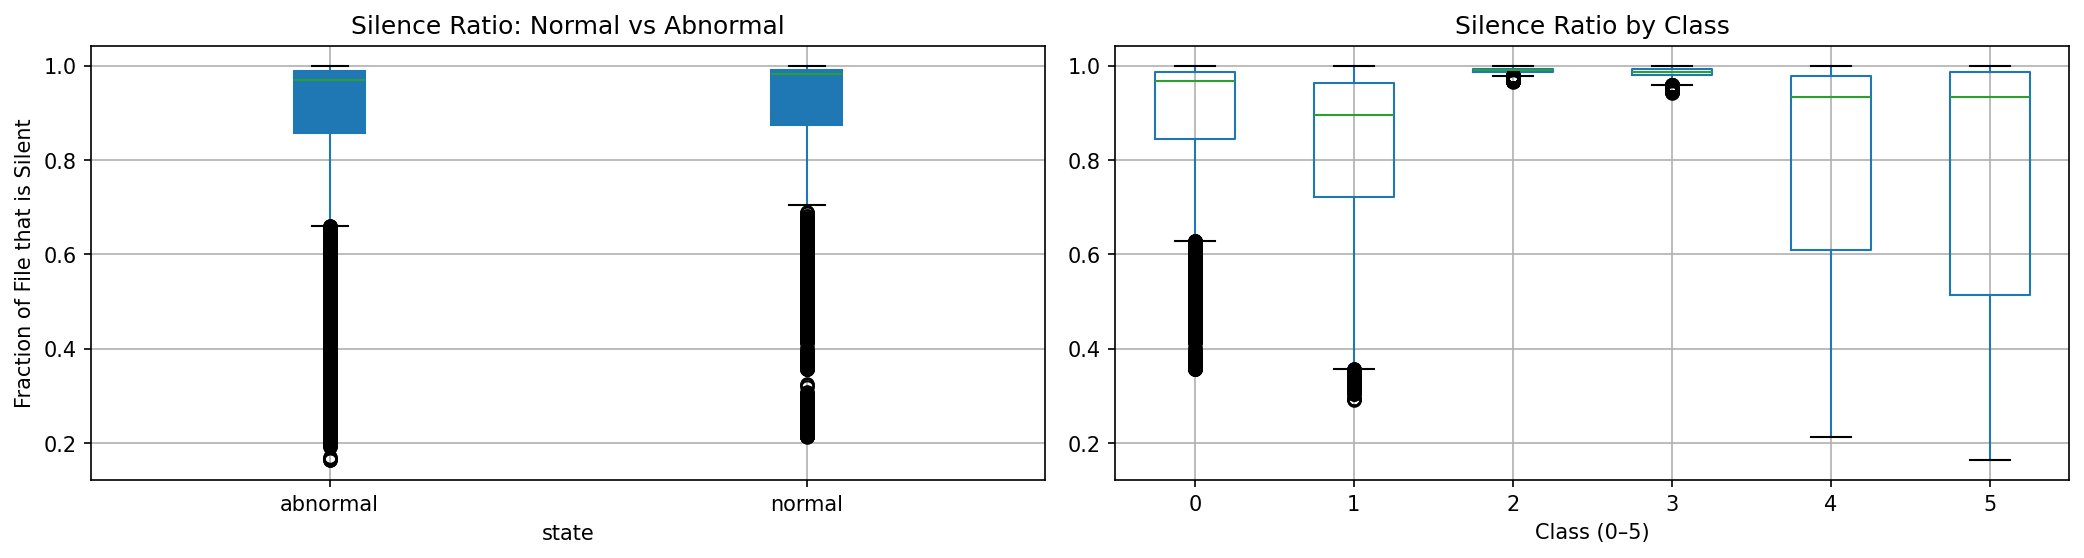
\includegraphics[width=0.7\textwidth]{figures/eda_silence.png}
    \caption{Silence Ratio Analysis across Machine States}
    \label{fig:silence_ratio}
\end{figure}

\section{Correlation Analysis}
We conducted a correlation analysis of basic acoustic features. We found that abnormal samples often have a higher Zero-Crossing Rate (ZCR) due to the increased mechanical noise and clatter associated with faults.

\section{High-Dimensional Visualization (t-SNE)}
To evaluate the inherent separability of the 100 extracted features, we employed t-Distributed Stochastic Neighbor Embedding (t-SNE). This non-linear dimensionality reduction technique allows us to visualize high-dimensional clusters in a 2D space while preserving local structures.

\begin{figure}[H]
    \centering
    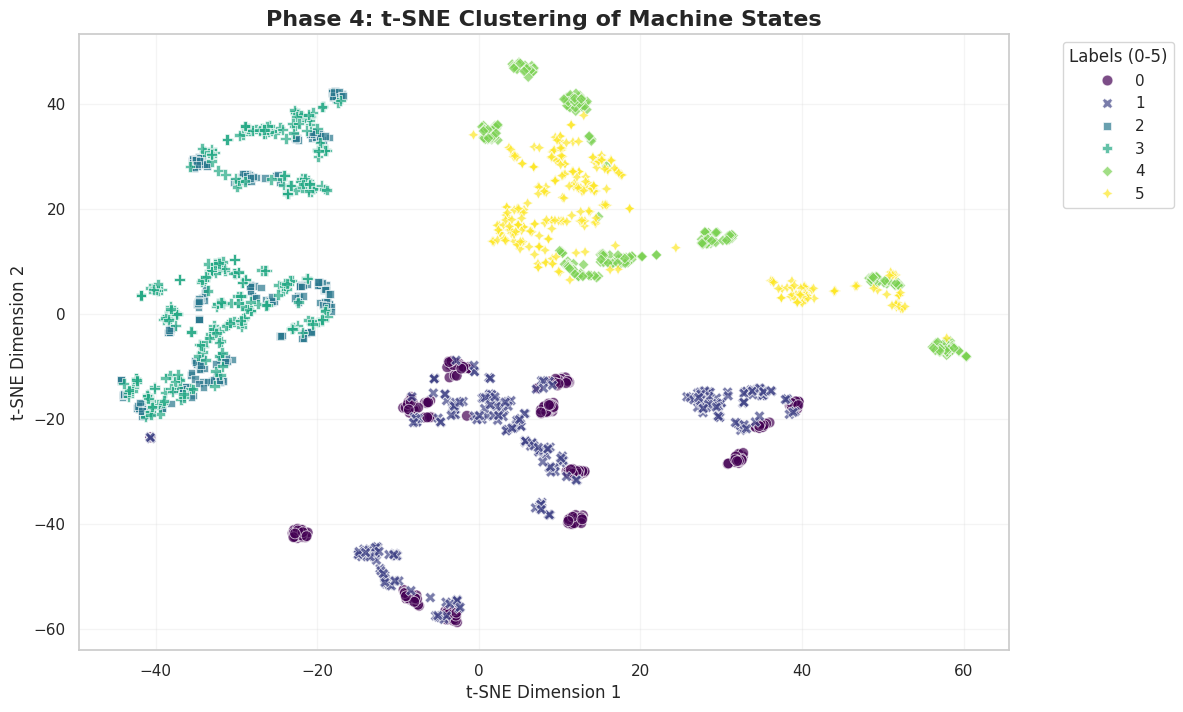
\includegraphics[width=0.8\textwidth]{figures/notebook_tsne_plot.png}
    \caption{t-SNE Projection of Acoustic Features across 6 Classes}
    \label{fig:tsne_plot}
\end{figure}

The t-SNE plot revealed distinct macro-clusters corresponding to each of the three machines, indicating that a machine's baseline mechanical signature is the most dominant acoustic feature. Crucially, within each machine-specific "island," the "Normal" and "Abnormal" samples exhibit clear sub-clustering and separation. This confirms that the hand-crafted acoustic manifold successfully captures both machine identity and fault status.

\section{Feature Inter-correlation}
Correlation heatmaps of the Top 15 features showed that while MFCCs are highly correlated with each other, Spectral Contrast and Zero-Crossing Rate provide independent information. This low inter-correlation between diverse feature families is why our hand-crafted acoustic manifold achieves high performance.

\begin{figure}[H]
    \centering
    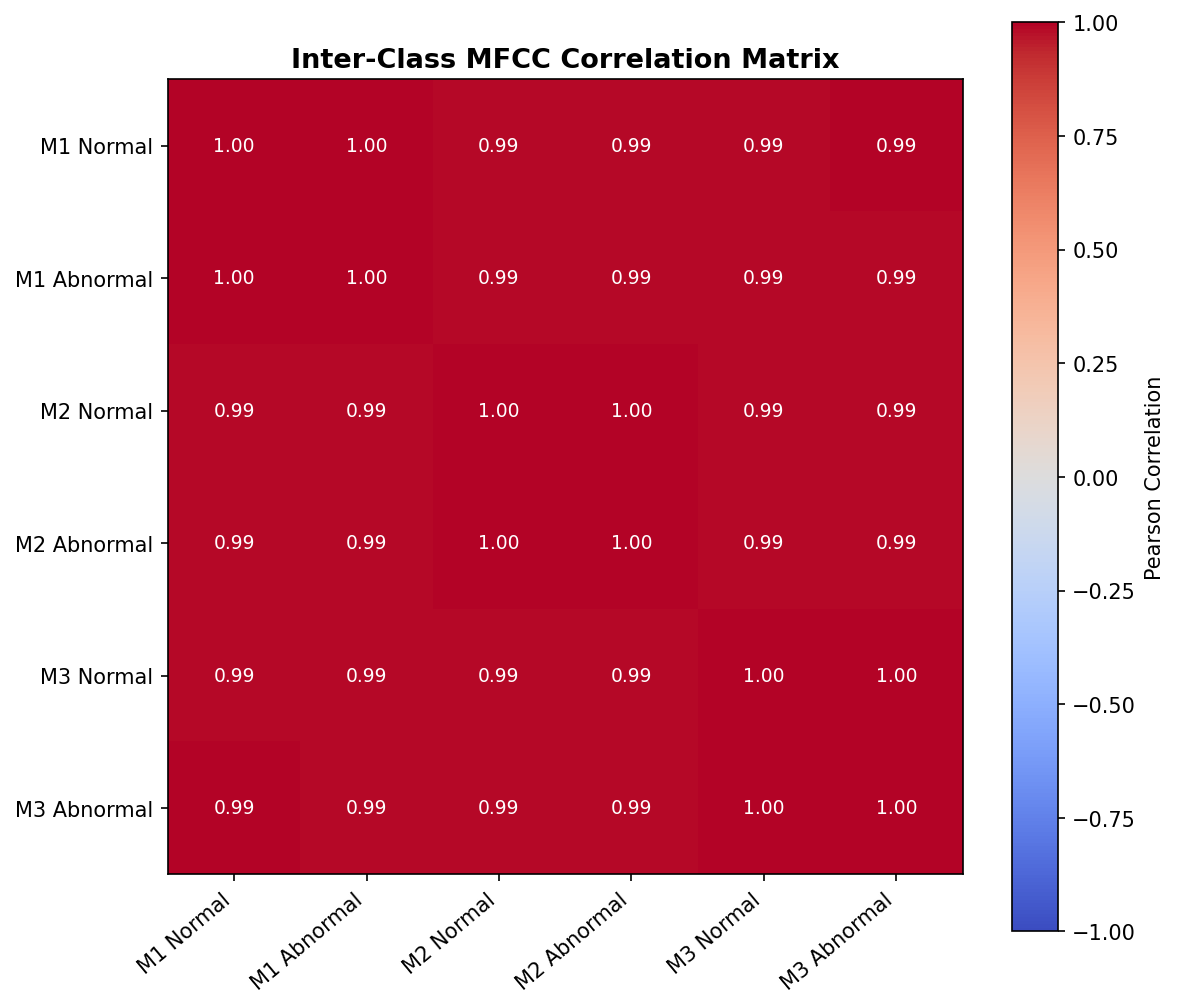
\includegraphics[width=0.7\textwidth]{figures/eda_correlation.png}
    \caption{Correlation Heatmap of Top Acoustic Features}
    \label{fig:corr_heatmap}
\end{figure}

\section{Machine-Specific Distinctions}
Boxplot analysis across Machines 1, 2, and 3 showed that while the absolute values of Spectral Centroid vary significantly between machines (due to different motor speeds), the \textit{relative shift} between Normal and Abnormal states remains consistent, providing a robust signature for anomaly detection.

\begin{figure}[H]
    \centering
    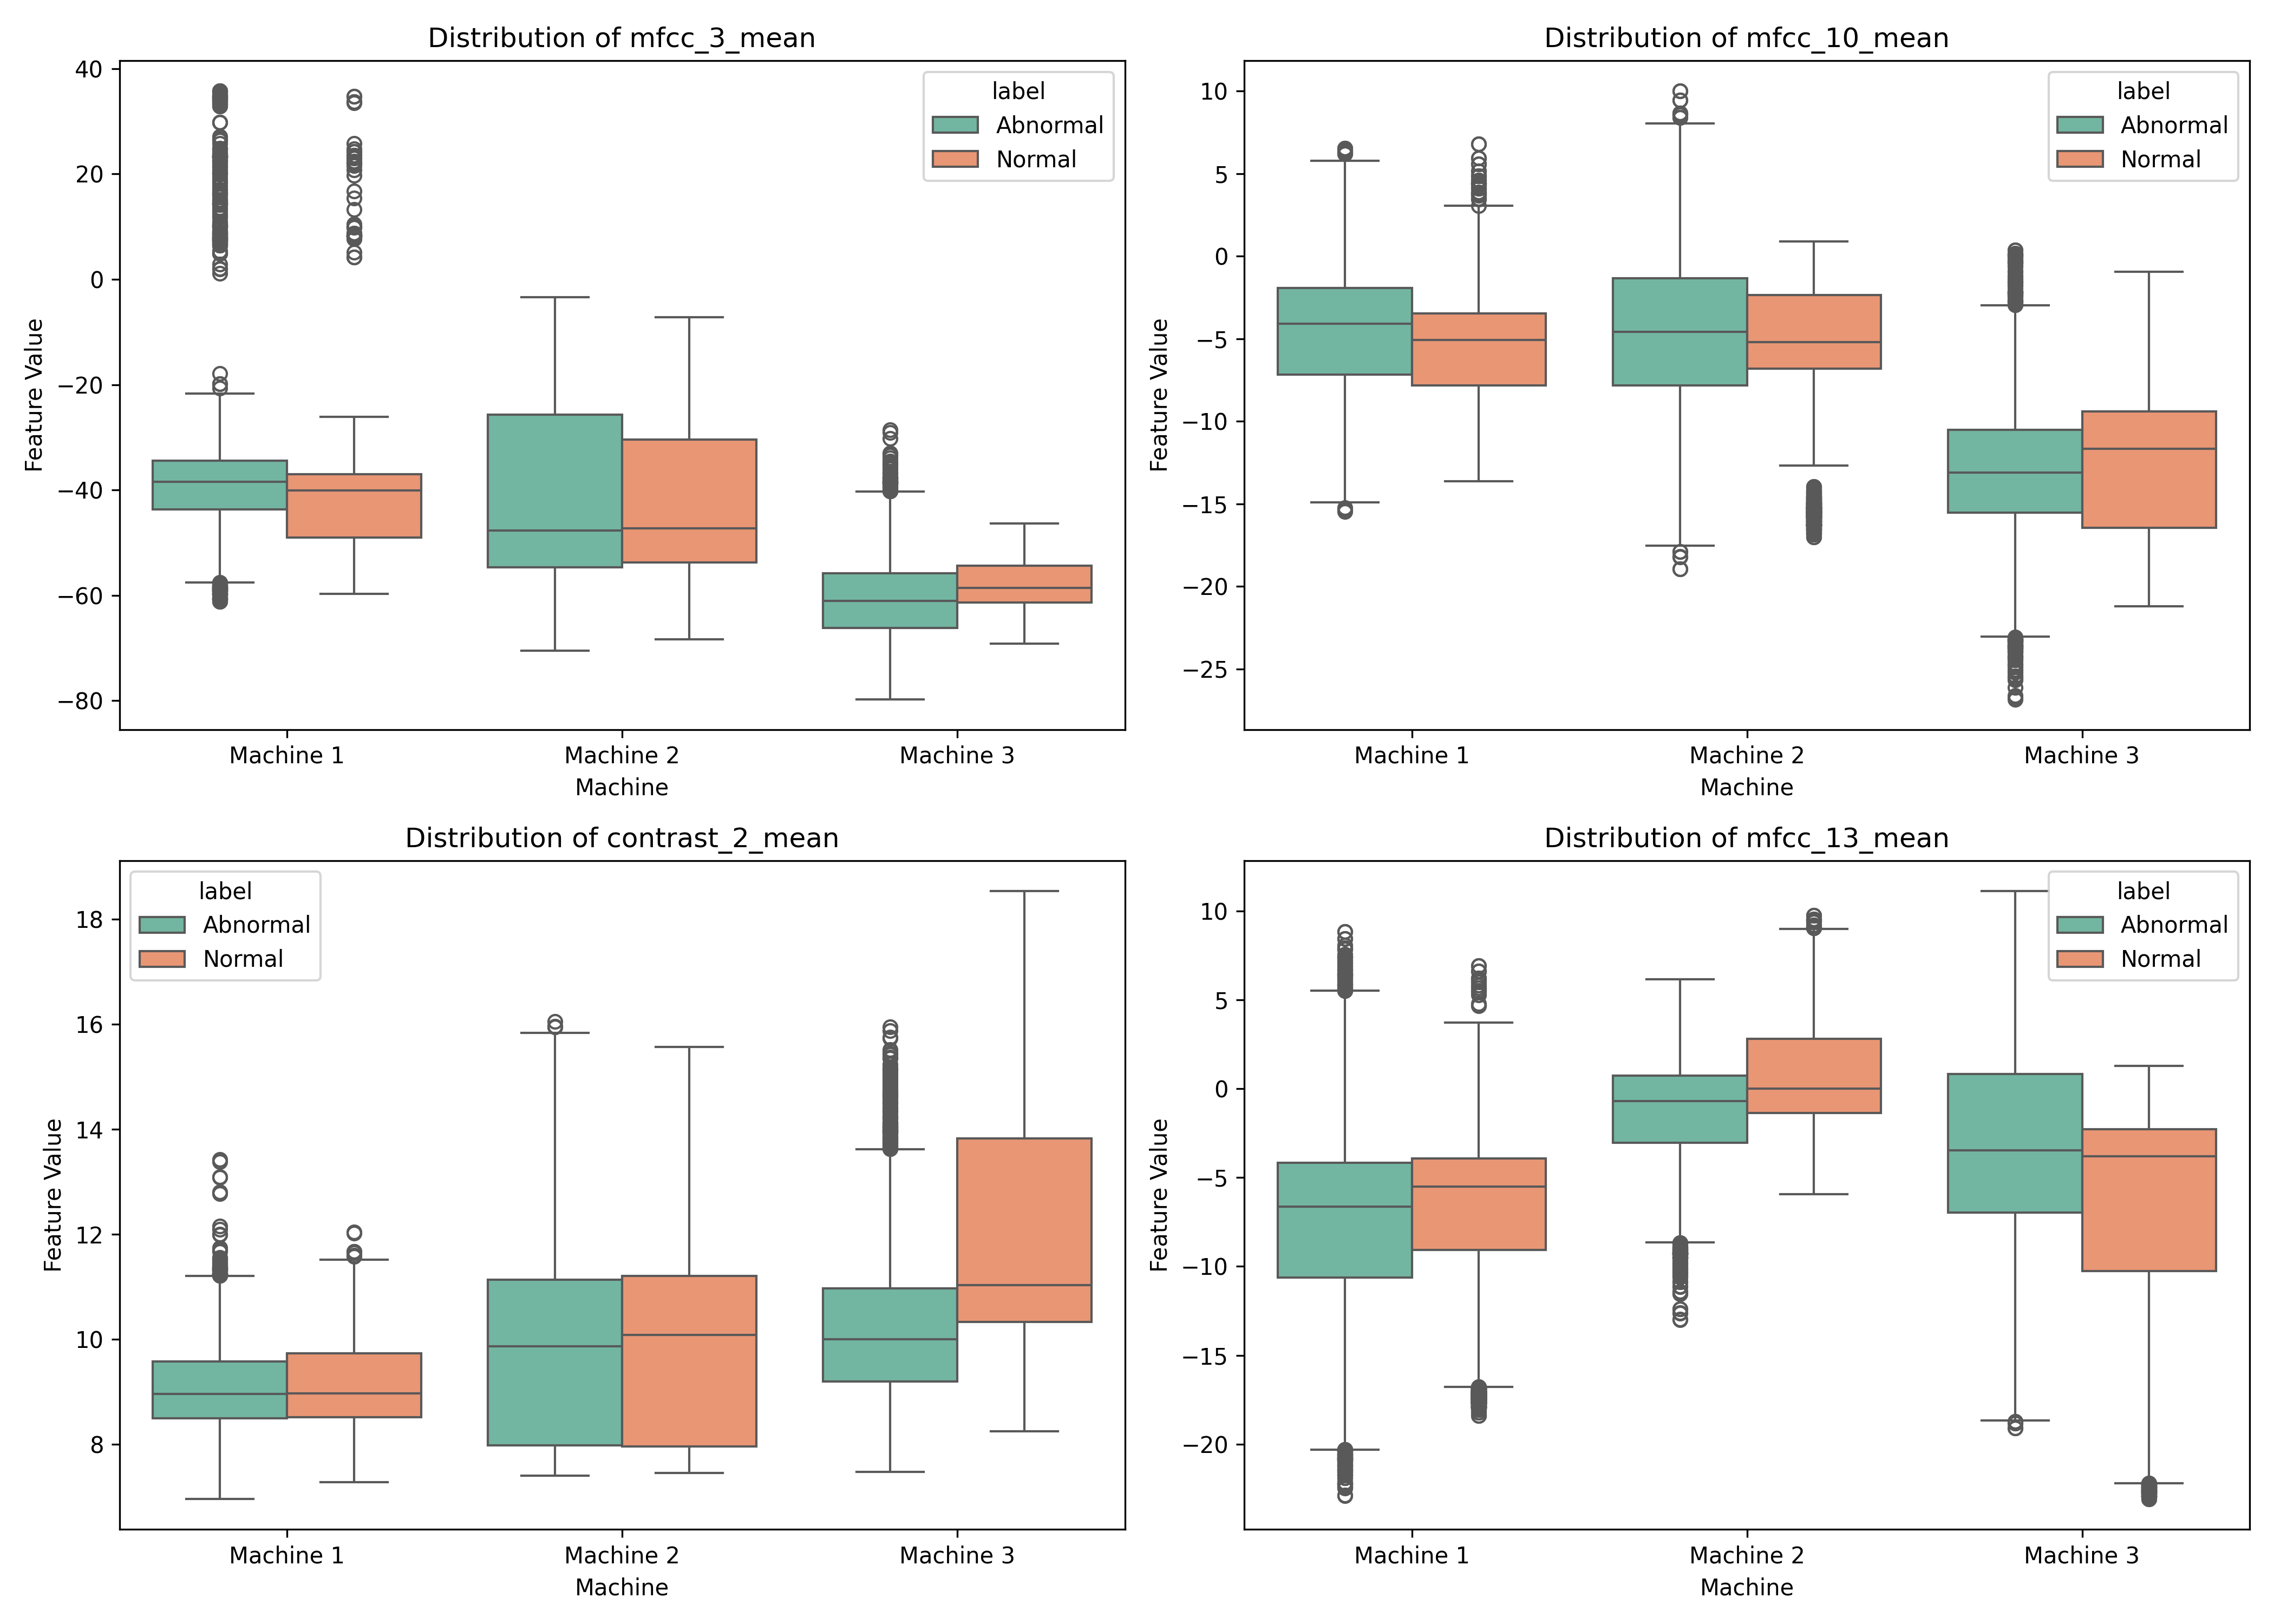
\includegraphics[width=0.7\textwidth]{figures/top_features_boxplot.png}
    \caption{Distribution of Top 4 Features across Machines}
    \label{fig:top_features_boxplot}
\end{figure}
